\newpage

\section{Two Neuron Connections}

Connectivity in local cortical circuits displays a distinctive
feature: Bidirectionally connected pairs of neurons appear much more
frequent than one would expect from the overall connection
probability. This aspect of local networks has been reported
repeatedly,

% Makram 1997, Song 2005.


% . First
% described by Markram 1997, finding across have confirmed . 

% A first result

% In anisotropic networks an overrepresentation of reciprocal
% connections is present. Counting and comparing it with our expectation
% from Gilbert random graphs $G(n,p)$, In random graphs the probabilities
% that a random pair of vertices are 

Here we investigate whether anisotropy in connectivity can be at cause
for this overrepresentation of reciprocally connected pairs. In random
networks, the chance to encounter a specific mode of connection in
a random pair of neurons be can easily be computed from the overall
connection probability $p$. For this let $X$ be the random variable of the
number of edges between two different vertices in a Gilbert graph
$G(n,p)$ with $n \ge 2$. As the edges are independently realized
resulting in a simple directed graph, we have
\begin{equation}
  \label{eq:pairs}
  \begin{aligned}%
    & \mathbf{P}(X=0) = (1-p)^2   &&\text{unconnected pair,}  \\
    & \mathbf{P}(X=1)= 2p(1-p)    &&\text{single connection,}\\
    & \mathbf{P}(X=2) = p^2       &&\text{reciprocal connection};
  \end{aligned}%
\end{equation}
in short $\mathbf{P}(X=k) = \mathcal{B}_{2,p}(k)$ for $k \in
\{0,1,2\}$ and $P(X=k) = 0$ otherwise. This probability distribution
reflects the expectation for connectivity of neuron pairs in
anisotropic networks. A numeric analysis of the anisotropic sample
graphs reveals that bidirectionally connected pairs appear almost
twice as often as expected from the overall connection
probability($p=0.116$) and equations \ref{eq:pairs}, similarly as
reported by Song et al.~(\autoref{fig:two_neuron_probs}
A). However, comparing pair probabilties in anisotropic networks with
the probabilities in their rewired counterparts we find that
anisotropy is does not influence the occurrence of two-neuron motifs
(\autoref{fig:two_neuron_probs} B) In fact, expected connections in
neuron pairs are identical in distance-dependent and rewired
anisotropic networks (\autoref{suppfig:two_neuron_dist_rew}).

\begin{figure}[ht]
  \centering
  \makebox{%
    \begin{overpic}[height=0.17\textheight]{%
        plots/c5f1462b_aniso_rand.pdf}
      \put(13.1,64.8){\small\textbf{A}}
      %\put(14.3,78.9){\small\textbf{A}}
    \end{overpic}
    \hspace{0.45cm}
    \begin{overpic}[height=0.17\textheight]{%
        plots/c5f1462b_aniso_rew.pdf}      
      \put(15.8,64.8){\small\textbf{B}}
    \end{overpic}
  }%
  \vspace{0.2cm}
  \caption{\textbf{Overrepresentation of reciprocal connections in
      anisotropic networks due to distance-dependent connectivity}
    Extracting the counts of unconnected, one-directionally and
    bidirectionally connected neuron pairs in the anisotropic sample
    graphs, overrepresentation of reciprocally connected pairs is
    identified as a feature of the network's distance dependency as
    opposed to anisotropy in connectivity. \textbf{A)} Showing the
    quotient of the counts for the three pair types, extracted from the
    set of sample graphs, with the number of expected pairs in Gilbert
    random graphs $G(n,p)$, where $n=1000$ and $p=0.116$ were matched
    to the sample graph parameters. While single connections appear
    less often than in Gilbert random graphs, reciprocal connections
    are significantly overrepresented. Errorbars SEM. \textbf{B)}
    Comparing appearance of connection pairs in the anisotropic sample
    graphs with their respective appearance in the rewired sample
    graphs, we find that eliminating anisotropy does not significantly
    change the counts for the connection types, indicating that
    anisotropy does not influence two neuron connection
    probabilities. Errorbars SEM.  (\smtcite{c5f1462b})}
  \label{fig:two_neuron_probs}
\end{figure}  




We can further support this observation by computing the probability
distribution for the expected number of edges between to random
vertices in the anisotropic graph model. Explicitly assuming that only
the distance-dependent connection probability $C(x)$ as calculated in
Theorem~\ref{theorem:distance_prof} is decisive in determining the
distribution for connections in neuron pairs, we can from $C(X)$ and
the probability distribution $f(x)$ for the a random neuron pair to be
at distance $x$ (Theorem~\ref{theorem:distance_square}), determine
\textbf{P}.
\begin{align*}
\mathbf{P}(X=0) & = \int_0^{\sqrt{2}} (1-C(x))^2 f(x)\,
dx, \\
\mathbf{P}(X=1) & = \int_0^{\sqrt{2}} 2 C(x) (1-C(x)) f(x) \, dx \quad \mathrm{and}\\
\mathbf{P}(X=2) & = \int_0^{\sqrt{2}} C(x)^2 f(x) \, dx 
\end{align*}
which yields, using the and
\begin{align*} 
\mathbf{P}(X=0) & = 0.791336 && 0.7907  \pm 0.0008\\
\mathbf{P}(X=1) & = 0.184151 && 0.1846  \pm 0.0007\\
\mathbf{P}(X=2) & = 0.024513 && 0.02462  \pm 0.00009
\end{align*}

% From Python c5f1462b
% Unconn:       0.790732332332  +- 0.000817274958369
% Single:       0.184638238238  +- 0.00074516663005
% Recip:        0.0246294294294  +- 8.63947164473e-05


% Mathematica (expected_two_neuron.nb)
% Unconn:       0.791336
% Single:       0.184151
% Recip:        0.024513 


Maybe simplicity of the model makes stuff wrong. Tune to Perin
distance profile.

Let 


\begin{figure}[htp]
  \centering
  \makebox{%
    \begin{overpic}[height=4.05cm]{%
        plots/6154302f.pdf}
      \put(85.5,57.5){\small\textbf{A}}
      %\put(12,5){\small\textbf{A}}
    \end{overpic}
    \hfill
    \begin{overpic}[height=4cm]{%
        plots/ef0e785d.pdf}
      \put(90.5,58.2){\small\textbf{B}}
    \end{overpic}
  }%
  \vspace{-0.15cm}
  \caption{ (\smtcite{6154302f}, \smtcite{ef0e785d})} %?? fix width issue!!
  \label{fig:determine_side_length}
\end{figure}

With side length 296:

% Mean:  0.115976056056
% Standard deviation:  0.00293436235458

from \smtcite{f11dca65}.


\begin{figure}[htp]
  \centering
  \makebox{%
    \begin{overpic}[width=0.5\textwidth]{%
        plots/875505b0_overall.pdf}
      \put(28,19){\small\textbf{A}}
    \end{overpic}
    \hfill
    \begin{overpic}[width=0.5\textwidth]{%
        plots/875505b0_single.pdf}
      \put(28,19){\small\textbf{B}}
    \end{overpic}
  }%
  \vspace{-0.6cm}
  \makebox{%
    \begin{overpic}[width=0.5\textwidth]{%
        plots/875505b0_recip.pdf}
       \put(28,19){\small\textbf{C}}
    \end{overpic}
    \vspace{-1cm}
    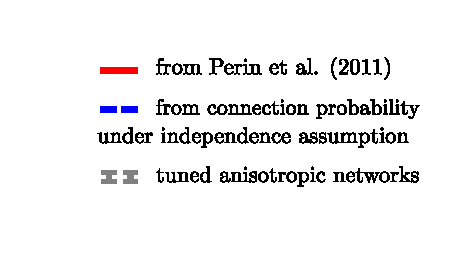
\includegraphics[width=0.5\textwidth]{%
      img/tuned_legend.pdf}   
  }%
  \vspace{-0.15cm}
  \caption{\textbf{Overrepresentation of reciprocal connections
      independent of } Comparison of occurrences of one- and
    bidirectionally connected neuron pairs in (gray) with profiles
    found by \textcite{Perin2011} (red), shows that overrepresentation of
    bidirectional pairs is distance-independent and not connected to
    anisotropy.  \textbf{A)} Overall connection probability in the
    adapted anisotropic networks was successfully tuned to reflect
    connection probability found by Perin et al. \textbf{B)-C)}
    Probabilities for a random neuron pair to display , 
    (\smtcite{875505b0})} %?? fix width issue!!
  \label{fig:perin_profiles_and_such}
\end{figure}


%%% Local Variables: 
%%% mode: latex
%%% TeX-master: "../dplths_document"
%%% End: 
